\section{Введение}
Задачи нелинейной глобальной оптимизации встречаются в различных прикладных областях \cite{Kvasov2013, Barkalov2013},
и традиционно считаются одними из самых трудоёмких среди оптимизационных задач.
Их сложность экспоненциально растёт в зависимости от размерности пространства поиска \cite{Vavasis1995},
поэтому для решения существенно многомерных задач требуются суперкомпьютерные вычисления и
экономичные алгоритмы оптимизации.

Вопрос ускорения сходимости актуален и для задач малой размерности в том случае, если вычисление
целевых функций задачи --- трудоёмкий процесс (например, в \cite{Barkalov2013} рассматривается
задача, в которой для проведения 400 вычислений двухмерной функции требуется 2,4 часа).
В такой ситуации важным свойством алгоритмов глобальной оптимизации является экономичность по
числу итераций. В рамках информационно-статичтического \cite{strOptBook} и геометрического подходов \cite{piyavskij1972} к
построению алгоритмов глобальной оптимизации рассматриваются две общие для этих подходов
стратегии учёта локальных свойств оптимизируемой функции, позволяющие существенно
снизить затраты на поиск \cite{sergLocalTuning}. Первый метод учёта локальных свойств
основан на построении оценок констант Липшица для подобластей поиска и ранее был
исследован в одномерном случае \cite{sergLocalTuning,nestedLocal}, и, частично, в многомерном \cite{strongSerg}.
Второй способ учёта локальных свойств заключается в применении метода локальной оптимизации в процессе глобального
поиска и последующем использовании результатов его работы глобальным методом. Эта стратегия
описана и исследована в одномерном случае в \cite{sergLocalTuning}. Обе стратегии
учёта локальных свойств будут рассмотрены в данной работе применительно к многомерному
обобщению метода глобального поиска Стронгина \cite{strOptBook}.

В настоящее время на кафедре МОиСТ активно ведётся разработка программной системы
для глобальной оптимизации функций многих вещественных переменных Globalizer.
Эта система включает в себя последние теоретические разработки, сделанные на кафедре в
этой сфере, в том числе и блочную многошаговую схему редукции размерности \cite{blockNested}.
Отличительной чертой ситемы является то, что, она может работать как на CPU, так на
разных типах ускорителей вычислений с высокой степенью параллельности (XeonPhi, GPU Nvidia) \cite{examinArtcle, examinphiArtcle}.

В данной работе будут описана прикладная задача оптимизации, решённая с помощью системы
Globalizer, а также проведено исследование нескольких способов ускорения сходимости
базового алгортима глобальной оптимизции, используемого в системе.

\section{Постановка задачи глобальной липшицевой оптимизации}
Одна из постановок задачи глобальной оптимизации звучит следующим образом: найти
глобальный минимум \(N\)-мерной функции \(\varphi(y)\) в гиперинтервале
\(D=\{y\in R^N:a_i\leqslant x_i\leqslant{b_i}, 1\leqslant{i}\leqslant{N}\}\).
Для построения оценки глобального минимума по конечному количеству вычислений
значения функции требуется, чтобы \(\varphi(y)\) удовлетворяла условию Липшица.
\begin{displaymath}
\label{task}
\varphi(y^*)=\min\{\varphi(y):y\in D\}
\end{displaymath}
\begin{displaymath}
\label{lip}
|\varphi(y_1)-\varphi(y_2)|\leqslant L\Vert y_1-y_2\Vert,y_1,y_2\in D,0<L<\infty
\end{displaymath}

Классической схемой редукции размерности для алгоритмов глобальной оптимизации является
использование разверток --- кривых, заполняющих пространство \cite{strOptBook}.
\begin{displaymath}
\label{cube}
\lbrace y\in R^N:-2^{-1}\leqslant y_i\leqslant 2^{-1},1\leqslant i\leqslant N\rbrace=\{y(x):0\leqslant x\leqslant 1\}
\end{displaymath}
На рис. \ref{fig:peano_curve} представлены построенные численно с низкой точностью развёртки на плоскости и
в трёхмерном пространстве.

\begin{figure}[ht]
    \centering
    \subfloat{{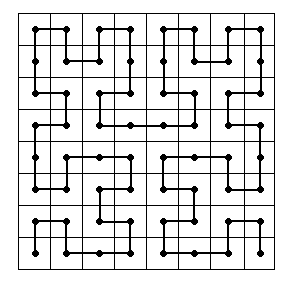
\includegraphics[width=0.45\textwidth]{images/peano2d.png} }}
    \qquad
    \subfloat{{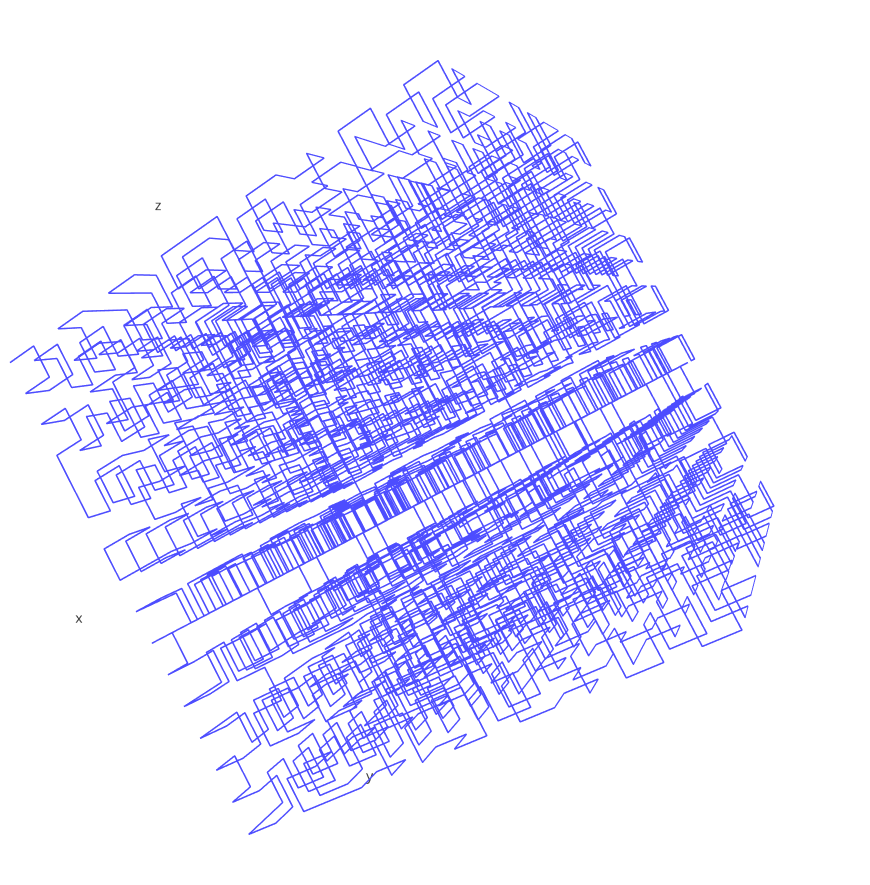
\includegraphics[width=0.45\textwidth]{images/peano3d.png} }}
    \caption{Численно построенная развёртка в двухмерном и трёхмерном случаях}
    \label{fig:peano_curve}
\end{figure}

Такое отображение позволяет свести задачу в многомерном пространстве к решению
одномерной ценой ухудшения её свойств. В частности, одномерная функция \(\varphi(y(x))\)
является не Липшицевой, а Гёльдеровой:
\begin{displaymath}
\label{holder}
|\varphi(y(x_1))-\varphi(y(x_2))|\leqslant H{|x_1-x_2|}^{\frac{1}{N}},x_1,x_2\in[0;1],
\end{displaymath}
где константа Гельдера \(H\) связана с константой Липшица \(L\) соотношением
\begin{displaymath}
H=4Ld\sqrt{N},d=\max\{b_i-a_i:1\leqslant i\leqslant N\}.
\end{displaymath}
На рис. \ref{fig:evolvent_example} приведена одномерная функция, полученная после применения развёртки к
парабалоиду вращения \(\varphi(y)=y_1^2+y_2^2\).

\begin{figure}[ht]
    \center
    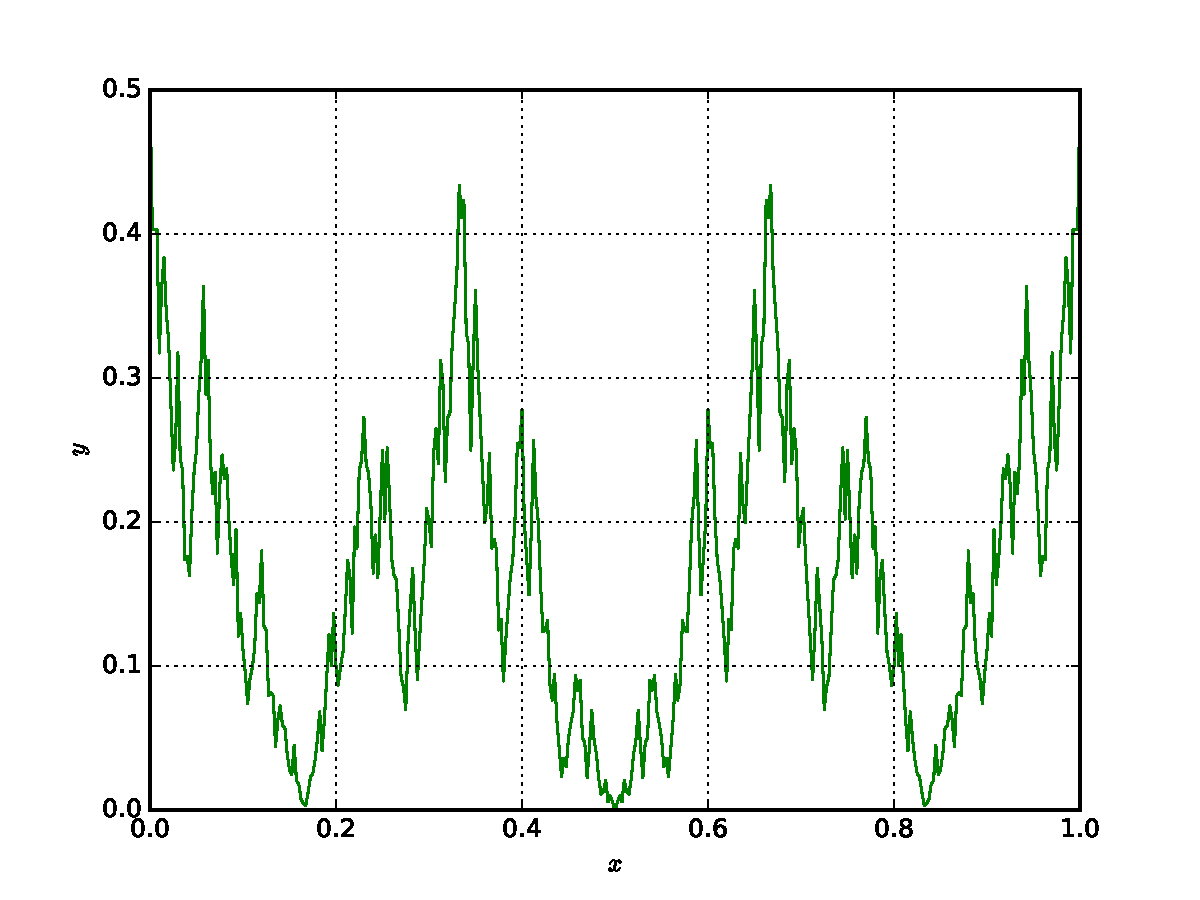
\includegraphics[width=0.75\textwidth]{images/map_paraboloid.pdf}
    \caption{Пример одномерной функции, порождённой развёрткой}
    \label{fig:evolvent_example}
\end{figure}

Область \(D\) также может быть задана с помощью функциональных ограничений.
Постановка задачи глобальной оптимизации в этом случае будет иметь следующий вид:
\begin{equation}
  \label{eq:constrained_problem}
  \varphi(y^*)=\min\{\varphi(y):g_j(y)\leqslant 0, 1\leqslant j\leqslant m\}
\end{equation}
Обозначим \(g_{m+1}(y)=f(y)\). Далее будем предполагать, что все функции \(g_k(y),1\leqslant k \leqslant m+1\)
удовлетворяют условию Липшица в некотором гиперинтервале, включающем \(D\).

\section{Алгоритм глобального поиска} \label{sec:method}
Для дальнейшего изложения потребуется описание метода глобальной оптимизации,
используемого в системе Globalizer. Многомерные задачи сводятся к одномерным с помощью
различных схем редукции размерности, поэтому можно рассматривать минимизацию одномерной
функции \(f(x), x\in[0;1]\), удовлетворяющей условию Гёльдера, при ограничениях, также
удовлетворяющих этому условию на интервале \([0;1]\).

Рассматриваемый алгоритм решения одномерной задачи (\ref{eq:constrained_problem}) предполагает построение последовательности
точек \(x_k\), в которых вычисляются значения минимизируемой функции или ограничений \(z_k = g_s(x_k)\).
Для учёта последних используется индексная схема \cite{strongSerg}. Пусть \(Q_0=[0;1]\). Ограничение, имеющее номер
 \(j\), выполняется во всех точках области
\begin{displaymath}
  Q_j=\left\{x\in [0;1]:g_j(x)\leq 0\right\},
\end{displaymath}
которая называется допустимой для этого ограничения. При этом допустимая область \(D\)
исходной задачи определяется равенством: \(D=\cap _{j=0}^{m}Q_{j}\).
Испытание в точке \(x\in [0;1]\) состоит в последовательном вычислении значений
величин \(g_{1}(x),...,g_{\nu }(x)\), где значение индекса \(\nu\) определяется условиями:
\(x\in Q_{j},0\leqslant j<\nu ,x\notin Q_{\nu }\). Выявление первого нарушенного ограничения
прерывает испытание в точке \(x\). В случае, когда точка \(x\)  допустима, т. е.
\(x\in D\) испытание включает в себя вычисление всех функций задачи. При этом значение
индекса принимается равным величине \(\nu =m+1\). Пара \(\nu =\nu (x),z=g_{\nu }(x)\),
где индекс \(\nu\) лежит в границах \(1\leqslant \nu \leqslant m+1\), называется результатом
испытания в точке \(x\).

Такой подход к проведению испытаний позволяет свести исходную задачу с функциональными
ограничениями к безусловной задаче минимизации разрывной функции:

\begin{displaymath}
  \begin{array}{lr}
    \psi (x^{*})=\min_{x\in [0;1]}\psi (x), \\
    \psi (x)={\begin{cases}g_{\nu }(x)/H_{\nu }&\nu <M\\(g_{M}(x)-g_{M}^{*})/H_{M}&\nu =M\end{cases}}
  \end{array}
\end{displaymath}

Здесь \(M=\max_{}^{}\left\{\nu (x):x\in [0;1]\right\}\), а \(g_{M}^{*}=\min _{}^{}\left\{g_{M}(x):x\in \cap _{i=0}^{M-1}Q_{i}\right\}\).
В силу определения числа \(M\), задача отыскания \(g_{M}^{*}\)
всегда имеет решение, а если \(M=m+1\), то \(g_{M}^{*}=f(x^{*})\).
Дуги функции \(\psi (x)\) гельдеровы на множествах \(\cap _{i=0}^{j}Q_{i},0\leq j\leq M-1\)
с константой 1, а сама \(\psi (x)\) может иметь разрывы первого рода на границах этих множеств.
Несмотря на то, что значения констант Гёльдера \(H_k\) и величина \(g_{M}^{*}\) заранее неизвестны,
они могут быть оценены в процессе решения задачи.

Множество троек \(\{(x_k,\nu_k,z_k)\}, 1\leqslant k\leqslant n\) составляет поисковую информацию,
накопленную методом после проведения \(n\) шагов.

На первой итерации метода испытание проводится в произвольной внутренней точке \(x_1\)
интервала \([0;1]\). Индексы точек 0 и 1 считаются нулевыми, значения \(z\) в
них не определены. Пусть выполнено \(k\geqslant 1\) итераций метода,
в процессе которых были проведены испытания в \(k\) точках \(x_i, 1\leqslant i\leqslant k\).
Тогда точкa \(x^{k+1}\) поисковых испытаний следующей \((k+1)\)-ой
итерации определяются в соответствии с правилами:

Шаг 1. Перенумеровать точки множества \(X_k=\{x^1,\dotsc,x^k\}\cup\{0\}\cup\{1\}\),
которое включает в себя граничные точки интервала \([0;1]\), а также точки предшествующих
испытаний, нижними индексами в порядке увеличения значений координаты, т.е.
\begin{displaymath}
0=x_0<x_1<\dotsc<x_{k+1}=1
\end{displaymath}
и сопоставить им значения \(z_{i}=g_{\nu }(x_{i}),\nu =\nu (x_{i}),i={\overline {1,k}}\).

Шаг 2. Для каждого целого числа \(\nu ,1\leqslant \nu \leqslant m+1\) определить соответствующее
ему множество \(I_{\nu }\) нижних индексов точек, в которых вычислялись значения
функций \(g_{\nu }(x)\):
\begin{displaymath}
  I_{\nu }=\{i:\nu (x_{i})=\nu ,1\leqslant i\leqslant k\},1\leq \nu \leqslant m+1,
\end{displaymath}
определить максимальное значение индекса \(M=\max\{\nu (x_{i}),1\leq i\leq k\}\).

Шаг 3. Вычислить текущие оценки для неизвестных констант Гёльдера:
\begin{equation}
  \label{step2}
  \mu _{\nu }=\max\{\frac{|g_{\nu }(x_{i})-g_{\nu }(x_{j})|}{(x_{i}-x_{j})^{\frac{1}{N}}}:i,j\in I_{\nu },i>j\}.
\end{equation}
Если множество \(I_{\nu }\) содержит менее двух элементов или если значение \(\mu _{\nu }\)
оказывается равным нулю, то принять \(\mu _{\nu }=1\).

Шаг 4. Для всех непустых множеств \(I_{\nu },\nu ={\overline {1,M}}\) вычислить оценки
\begin{displaymath}
  z_{\nu }^{*}={\begin{cases}\min\{g_{\nu }(x_{i}):x_{i}\in I_{\nu }\}&\nu =M\\-\varepsilon _{\nu }&\nu <M\end{cases}},
\end{displaymath}
где вектор с неотрицательными координатами \(\varepsilon _{R}=(\varepsilon _{1},..,\varepsilon _{m})\) называется вектором резервов.

Шаг 5. Для каждого интервала \((x_{i-1};x_{i}),1\leqslant i\leqslant k\) вычислить характеристику
\begin{equation}
  \label{step3_1}
  R(i)={\begin{cases}\Delta _{i}+{\frac {(z_{i}-z_{i-1})^{2}}{(r_{\nu }\mu _{\nu })^{2}\Delta _{i}}}-2{\frac {z_{i}+z_{i-1}-2z_{\nu }^{*}}{r_{\nu }\mu _{\nu }}}&\nu =\nu (x_{i})=\nu (x_{i-1})\\2\Delta _{i}-4{\frac {z_{i-1}-z_{\nu }^{*}}{r_{\nu }\mu _{\nu }}}&\nu =\nu (x_{i-1})>\nu (x_{i})\\2\Delta _{i}-4{\frac {z_{i}-z_{\nu }^{*}}{r_{\nu }\mu _{\nu }}}&\nu =\nu (x_{i})>\nu (x_{i-1})\end{cases}}
\end{equation}
где \(\Delta _{i}=(x_{i}-x_{i-1})^{\frac{1}{N}}\). Величины \(r_{\nu }>1,\nu ={\overline {1,m}}\)
являются параметрами алгоритма. От них зависят произведения \(r_{\nu }\mu _{\nu }\),
используемые при вычислении характеристик в качестве оценок неизвестных констант Гёльдера.

Шаг 5. Выбрать наибольшую характеристику:
\begin{equation}
\label{step4}
t=\argmax_{1\leqslant i \leqslant k+1}R(i)
\end{equation}

Шаг 6. Провести очередное испытание в середине интервала \((x_{t-1};x_{t})\),
если индексы его концевых точек не совпадают: \(x^{k+1}={\frac {1}{2}}(x_{t}+x_{t-1})\).
В противном случае провести испытание в точке
\begin{displaymath}
  x^{k+1}={\frac {1}{2}}(x_{t}+x_{t-1})-\operatorname {sgn}(z_{t}-z_{t-1}){\frac {|z_{t}-z_{t-1}|^{n}}{2r_{\nu }\mu _{\nu }^{n}}},\nu =\nu (x_{t})=\nu (x_{t-1}),
\end{displaymath}
а затем увеличить \(k\) на 1.

Алгоритм прекращает работу, если выполняется условие \(\Delta_{t}\leqslant \varepsilon\),
где \(\varepsilon>0\) есть заданная точность. В качестве оценки глобально-оптимального решения задачи  выбираются значения
\begin{equation}
f_k^*=\min_{1\leqslant i \leqslant k}f(x_i), x_k^*=\argmin_{1\leqslant i \leqslant k}f(x_i)
\end{equation}

Достаточные условия сходимости метода определяются следующей теоремой:
\begin{theorem}
  Пусть исходная задача оптимизации имеет решение \(x^{*}\) и выполняются следующие условия:
  \begin{itemize}
    \item каждая область \(Q_{j},j={\overline {1,m}}\) представляет собой объединение
    конечного числа отрезков, имеющих положительную длину;
    \item каждая функция \(g_{j}(x),j={\overline {1,m+1}}\) удовлетворяет условию Гёльдера с соответствующей константой \(H_{j}\);
    \item компоненты вектора резервов удовлетворяют неравенствам \(0\leq 2\varepsilon _{\nu }<L_{\nu }(\beta -\alpha )\),
    где \(\beta -\alpha\) --- длина отрезка \([\alpha ;\beta ]\), лежащего в допустимой области \(D\) и содержащего точку \(x^{*}\);
    \item начиная с некоторого значения \(k\) величины \(\mu _{\nu }\), соответствующие
    непустым множествам \(I_{\nu }\), удовлетворяют неравенствам \(r_{\nu }\mu _{\nu }>2H_{\nu }\).
  \end{itemize}
  Тогда верно следующее:
  \begin{itemize}
    \item точка \(x^{*}\) является предельной точкой последовательности \(\{x^{k}\}\), порождаемой методом при \(\varepsilon =0\)  в условии остановки;
    \item любая предельная точка \(x^{0}\)  последовательности \(\{x^{k}\}\) является решением исходной задачи оптимизации;
    \item сходимость к предельной точке \(x^{0}\) является двухсторонней, если \(x^{0}\not =a,x^{0}\not =b\).
  \end{itemize}
\end{theorem}

Подробнее метод и теорема о его сходимости описаны в \cite{strongSerg}.

\subsection{Сравнение методов оптимизации} \label{subsec:methods_compasion}
Существует несколько критериев оптимальности алгоритмов поиска (минимаксный, критерий
одношаговой оптимальности), но большинстве случаев представляет интерес
сравнение методов по среднему результату, достижимому на конкретном подклассе липшицевых функций.
Достоинством такого подхода является то, что средний показатель можно оценить
по конечной случайной выборке задач, используя методы математической статистики.

В качестве оценки эффективности алгоритма будем использовать, операционную характеристику,
которая определяется множеством точек на плоскости \((K, P)\),
где \(K\) – среднее число поисковых испытаний, предшествующих выполнению условия
остановки при минимизации функции из данного класса, а \(P\) – статистическая вероятность того,
что к моменту остановки глобальный экстремум будет найден с заданной точностью.
Если при выбранном \(K\) операционная характеристика одного метода лежит выше характеристики другого,
то это значит, что при фиксированных затратах на поиск первый метод найдёт решение с
большей статистической вероятностью. Если же зафиксировать некоторое значение \(P\), и
характеристика одного метода лежит левее характеристики другого, то первый метод
требует меньше затрат на достижение той же надёжности.

\subsection{Классы тестовых задач} \label{subsec:test_problems}
Для сравнения алгоритмов глобального поиска в смысле операционной характеристики
требуется иметь некоторое множество тестовых задач. Генератор задач GKLS, описанный в
\cite{gklsBook} позволяет получить такое множество задач с заренее известными свойствами.
Это достигается за счёт модификации параболоида \(g(x)=\Vert x-T\Vert + t\) в
шаровых окрестностях некоторых случайно сгенерированных точек \(M_i, i=\overline{1,m}\). В точках
\(M_i\) распологаются локальные минимумы со значениями, превосходящими значение
\(g(T)=t\). Таким образом, координаты глобального минимума в задачах GKLS всегда заведомо известны.
В данной работе используется несколько классов, сгенерированный GKLS: 2d Simple, 4d Simple и 5d Simple,
параметры которых также описаны в \cite{gklsBook}. Функции рассматриваемых
классов являются непрерывно дифференцируемыми и имеют 10 локальных минимумов, один из которых является глобальным.

Ещё одним тестовым классом, используемым в данной работе для сравнения методов,
является набор двухмерных функций, предложенных В. А. Гришагиным \cite{grishaginClass}.
Каждая функция существенно многоэкстремальна и задаётся формулой:

\begin{displaymath}
  \varphi(y)=\sqrt{\left(\sum_{i=1}^7\sum_{j-1}^7 A_{ij}g_{ij}(y)+ B_{ij}h_{ij}(y)\right)^2+\left(\sum_{i=1}^7\sum_{j-1}^7 C_{ij}g_{ij}(y) - D_{ij}h_{ij}(y)\right)^2}
\end{displaymath}
где
\begin{displaymath}
  \begin{array}{cr}
    y\in[0;1]^2, \\
    g_{ij}=\sin(i\pi y_1)\sin(j\pi y_2), \\
    h_{ij}=\cos(i\pi y_1)\cos(j\pi y_2),
  \end{array}
\end{displaymath}
где коэффициенты \(A_{ij},B_{ij}, C_{ij}, D_{ij}\) генерируются случайно с равномерным в
интервале \([-1;1]\) распределением.
